% !TEX program = xelatex
\documentclass[a4paper]{article}
\usepackage{amsmath}
\usepackage{amsthm}
\usepackage[left=1.8cm,right=1.8cm,top=2.2cm,bottom=2.0cm]{geometry}
\usepackage{ctex}
\usepackage{enumerate}
\usepackage{fancyhdr}
\usepackage{xpatch}
\usepackage{graphicx} 
\usepackage{float} 
\usepackage{subfigure} 
\usepackage{amsfonts}
\usepackage{mathtools}
\usepackage{framed}
\usepackage{multicol}
\usepackage{listings}
\usepackage{hyperref}
\usepackage{tikz}
\usetikzlibrary{automata,positioning}
\theoremstyle{definition}
\newtheorem*{solution*}{\textbf{Solution:}}
\newtheorem*{proof*}{\textbf{Proof:}}
\newtheorem{theorem}{Theorem}[subsection]
\newtheorem{definition}{Definition}[subsection]
\newtheorem{lemma}{Lemma}[subsection]
\makeatletter

\AtBeginDocument{\xpatchcmd{\@thm}{\thm@headpunct{.}}{\thm@headpunct{}}{}{}}
\makeatother

\pagestyle{fancy}
\renewcommand{\baselinestretch}{1.15}

\usepackage{paralist}
\let\itemize\compactitem
\let\enditemize\endcompactitem
\let\enumerate\compactenum
\let\endenumerate\endcompactenum
\let\description\compactdesc
\let\enddescription\endcompactdesc

% shorten footnote rule
\xpatchcmd\footnoterule
  {.4\columnwidth}
  {1in}
  {}{\fail}

\title{CS 131 Compilers: Discussion 3: Top-Down Parsers}
\author{\textbf{杨易为}~~\textbf{季杨彪}~~\textbf{尤存翰} \\ \texttt{ \{yangyw,jiyb,youch\}@shanghaitech.edu.cn}}



\begin{document}
\maketitle
\section{DFA and NFA}
\subsection{Introduction}

Finite state automata (FSA) are abstract machines that feature states and guarded tran-sitions from one state to another.  An FSA can only be in one state a time, and its totalnumber of states isfinite.  The machine takes transitions in response to inputs it receivessequentially;  if an input matches the guard of a transition that departs from the currentstate that transition is said to beenabled; only enabled transitions can be taken.  FSA thathave an accepting state provide the machinery to determine whether an input string is in aregular language.  If no transitions are enabled by a given input then the entire input stringgets  rejected.   If  all  inputs  are  processed  and  the  FSA  is  in  an  accepting  state  then  theentire input string is accepted.  Deterministic finite state automata (DFA) can only haveone enabled transition at a time while a non-deterministic finite state automata (NFA) canhave multiple.

\subsection{What language is accepted by the following DFA?}
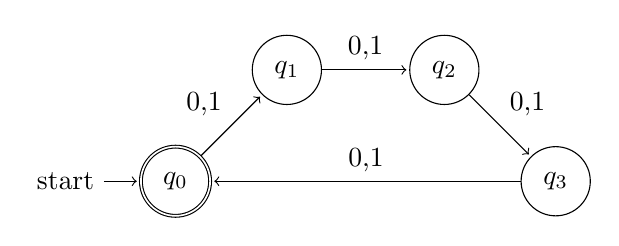
\begin{tikzpicture}[shorten >=1pt,node distance=2cm,on grid,auto]
    \node[state,initial,accepting] (q_0)   {$q_0$};
    \node[state] (q_1) [above right=of q_0] {$q_1$};
    \node[state] (q_2) [right=of q_1] {$q_2$};
    \node[state] (q_3) [below right=of q_2] {$q_3$};
    \path[->]
    (q_0) edge  node {0,1} (q_1)
    (q_1) edge  node  {0,1} (q_2)
    (q_2) edge  node  {0,1} (q_3)
    (q_3)edge  node  [above]{0,1} (q_0);

\end{tikzpicture}
\\
\textbf{Answer:}

\subsection{What language is accepted by the following NFA?}
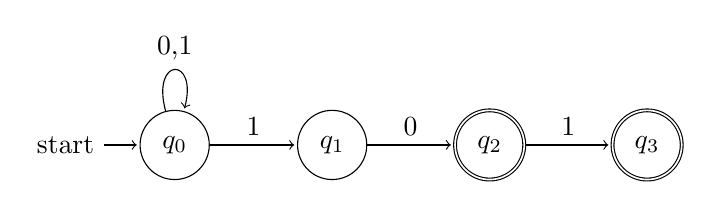
\begin{tikzpicture}[shorten >=1pt,node distance=2cm,on grid,auto]
    \node[state,initial] (q_0)   {$q_0$};
    \node[state] (q_1) [ right=of q_0] {$q_1$};
    \node[state,accepting] (q_2) [right=of q_1] {$q_2$};
    \node[state,accepting] (q_3) [ right=of q_2] {$q_3$};
    \path[->]
    (q_0) edge [loop above] node {0,1} ()
        edge  node  [above]{1} (q_1)
    (q_1) edge  node  {0} (q_2)
    (q_2) edge  node  {1} (q_3);

\end{tikzpicture}
\\
\textbf{Answer:}

\subsection{What language is accepted by the following NFA?}
\begin{tikzpicture}[shorten >=1pt,node distance=2cm,on grid,auto]
    \node[state,initial,accepting] (q_0)   {$q_0$};
    \node[state] (q_3) [ right=of q_2] {$q_3$};
    \node[state,accepting] (q_2) [right=of q_1] {$q_2$};
    \node[state,accepting] (q_1) [ right=of q_0] {$q_1$};
    \node[state,accepting] (q_4) [ right=of q_3] {$q_4$};
    \node[state,accepting] (q_5) [ right=of q_4] {$q_5$};
    \path[->]
    (q_0) 
        edge  node  [above]{0,1} (q_1)
    (q_1) edge  node  {0,1} (q_2)
    (q_2) edge  node  {0,1} (q_3)
    (q_3) edge  node  {0,1} (q_4)
    (q_4) edge  node  {0,1} (q_5)
    (q_5) edge [loop above] node {0,1} ();
\end{tikzpicture}
\\
\textbf{Answer:}


\subsection{Construct the NFA that accepts}
\subsubsection{$x(zy?|(yz)*)$}
\textbf{Answer:}
\subsubsection{$(10)*1*01*0$}
\textbf{Answer:}

\subsection{Minimized the NFA}
  \begin{enumerate}
	\item Original NFA, $\Sigma = \{a, b, c\}$:
	\\
	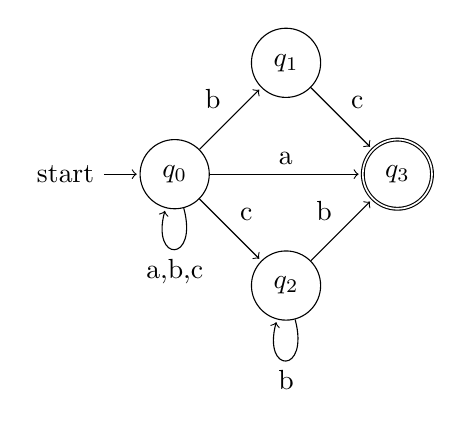
\begin{tikzpicture}[shorten >=1pt,node distance=2cm,on grid,auto]
		\node[state,initial] (q_0)   {$q_0$};
		\node[state] (q_1) [above right=of q_0] {$q_1$};
		\node[state] (q_2) [below right=of q_0] {$q_2$};
		\node[state,accepting](q_3) [below right=of q_1] {$q_3$};
		\path[->]
		(q_0) edge [loop below] node {a,b,c} ()
			  edge  node  [above] {a} (q_3)
			  edge  node  {b} (q_1)
			  edge  node  {c} (q_2)
		(q_1) edge  node  {c} (q_3)
		(q_2) edge  node  {b} (q_3)
			  edge  [loop below] node  {b} ();
	\end{tikzpicture}

\textbf{Answer:}
$
\\
\\
\\
\\
\\
$
\section{Pumpingg Lemma}
Pumping Lemma: For any DFA (or NFA or regular expression) that accepts an
infinite number of strings, there is some minimum length, \(M,\) such that any string
with length greater than or equal to \(M\) that the machine accepts must have the form
\(u x v,\) where \(u, x,\) and \(v\) are strings, \(x\) is not empty, the length of \(u x\) is \(\leq M,\) and the
machine accepts all strings of the form \(u x^{n} v,\) for all \(n \geq 0\).
\subsection{Proof of not regular} Let \(A=\left\{1^{j} z \mid z \in\{0,1\}^{*}\right.\) and \(z\) contains at most \(j\) i's, for any \(\left.j \geq 1\right\} .\) Prove, by the
pumping lemma, that \(A\) is not regular.\\
\textbf{Answer:}
$
\\
\\
\\
\\
\\
$
http://pfmiles.github.io/blog/left-recursion-removal-using-kleene-closure/

\end{document}
